\begin{figure}
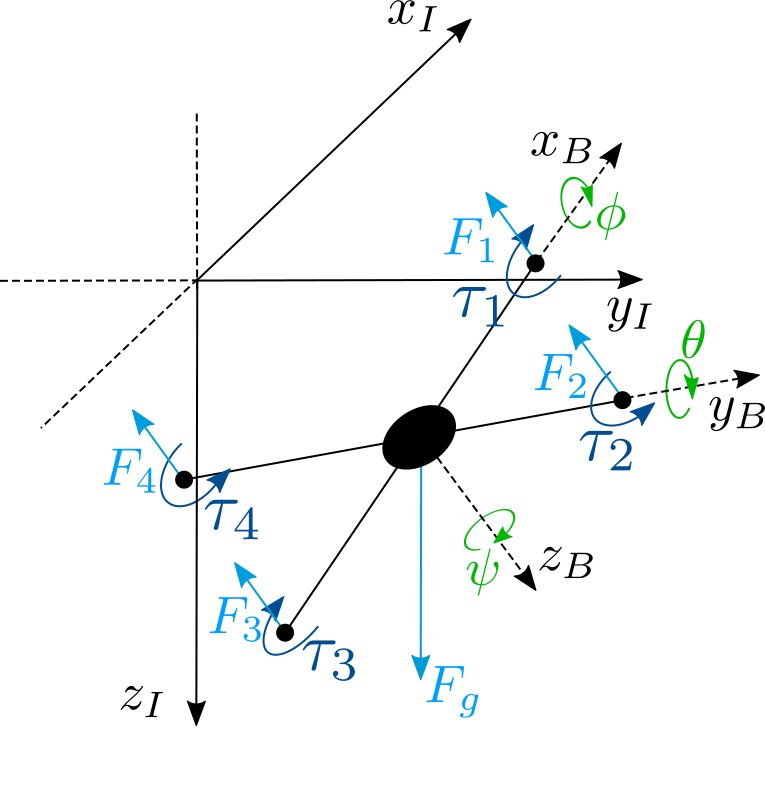
\includegraphics[width=0.7\linewidth]{figures/droneDiagram.pdf}
\caption{Free body diagram of the quadcopter along with the inertial and body coordinate systems.}
\end{figure}
\begin{itemize}
	\item Attitude model equations
\begin{flalign}
J_x\ddot{\phi}&=k_{\mathrm{th}} (\omega^2_4-\omega^2_2)  L \label{eq:AngleEqVelocities1}\\
J_y\ddot{\theta}&=k_{\mathrm{th}} (\omega^2_1-\omega^2_3)  L \label{eq:AngleEqVelocities2} \\
J_z\ddot{\psi}&=k_{\mathrm{d}} (\omega^2_1-\omega^2_2+\omega^2_3-\omega^2_4)\label{eq:AngleEqVelocities3}
\end{flalign}
\item Translational model equations
\begin{flalign}
m\ddot{x}_{\mathrm{I}} = &-k_{\mathrm{th}} ({\omega_1}^2+{\omega_2}^2+{\omega_3}^2+{\omega_4}^2) \label{eq:AccelerationEqInertial1}\\
& \ \times (\cos\phi \sin\theta \cos\psi + \sin\phi\sin\psi)   \nonumber\\
m \ddot{y}_{\mathrm{I}} = &-k_{\mathrm{th}}({\omega_1}^2+{\omega_2}^2+{\omega_3}^2+{\omega_4}^2) \label{eq:AccelerationEqInertial2}\\
& \ \times(\cos\phi \sin\theta \sin\psi - \sin\phi \cos\psi)  \nonumber\\
m\ddot{z}_{\mathrm{I}} = &F_g-k_{\mathrm{th}}\ ({\omega_1}^2+{\omega_2}^2+{\omega_3}^2+{\omega_4}^2) \label{eq:AccelerationEqInertial3}\\
& \ \times \cos\phi\cos\theta  \nonumber
\end{flalign}
\end{itemize}